\chapter{The LUX-ZEPLIN Dark Matter Experiment}
The LZ experiment is currently the leading dark matter direct detection experiment in the search for WIMPs. The detector is located on the 4,850~ft level (4,300~mwe) of the Sanford Underground Research Facility (SURF) in the Homestake Mine (Lead, SD) \cite{LZNIMA}. At the core of the experiment is a dual-phase Time Projection Chamber (TPC) which is sensitive to low -energy nuclear recoils (NR), the signal which is produced through WIMPs interacting with liquid noble gases. One of the main backgrounds in a WIMP search are neutrons as they also interact through nuclear recoils and thus LZ employs an active veto system to remove them. Theoretically WIMPs will only interact with the xenon target however neutrons would interact in both the TPC and veto detectors. The TPC is housed within a vacuum insulated cyrostat with a layer of liquid xenon (Skin) which acts as high voltage stand-off, this region is also instrumented with PMTs and is part of the active veto system. The LXe skin is used to veto mostly gamma ray interactions within the TPC volume, also being sensitive to neutrons. The cryostat is surrounded near hermetically by ten acrylic vessels filled with Gadolinium-loaded liquid scintillator (GdLS). The GdLS is observed by 120 PMTs and stands within 238t of DI water which provides shielding to the detector. A schematic of the detector is shown in \autoref{fig:LZDetector}.
\begin{figure}
    \centering
    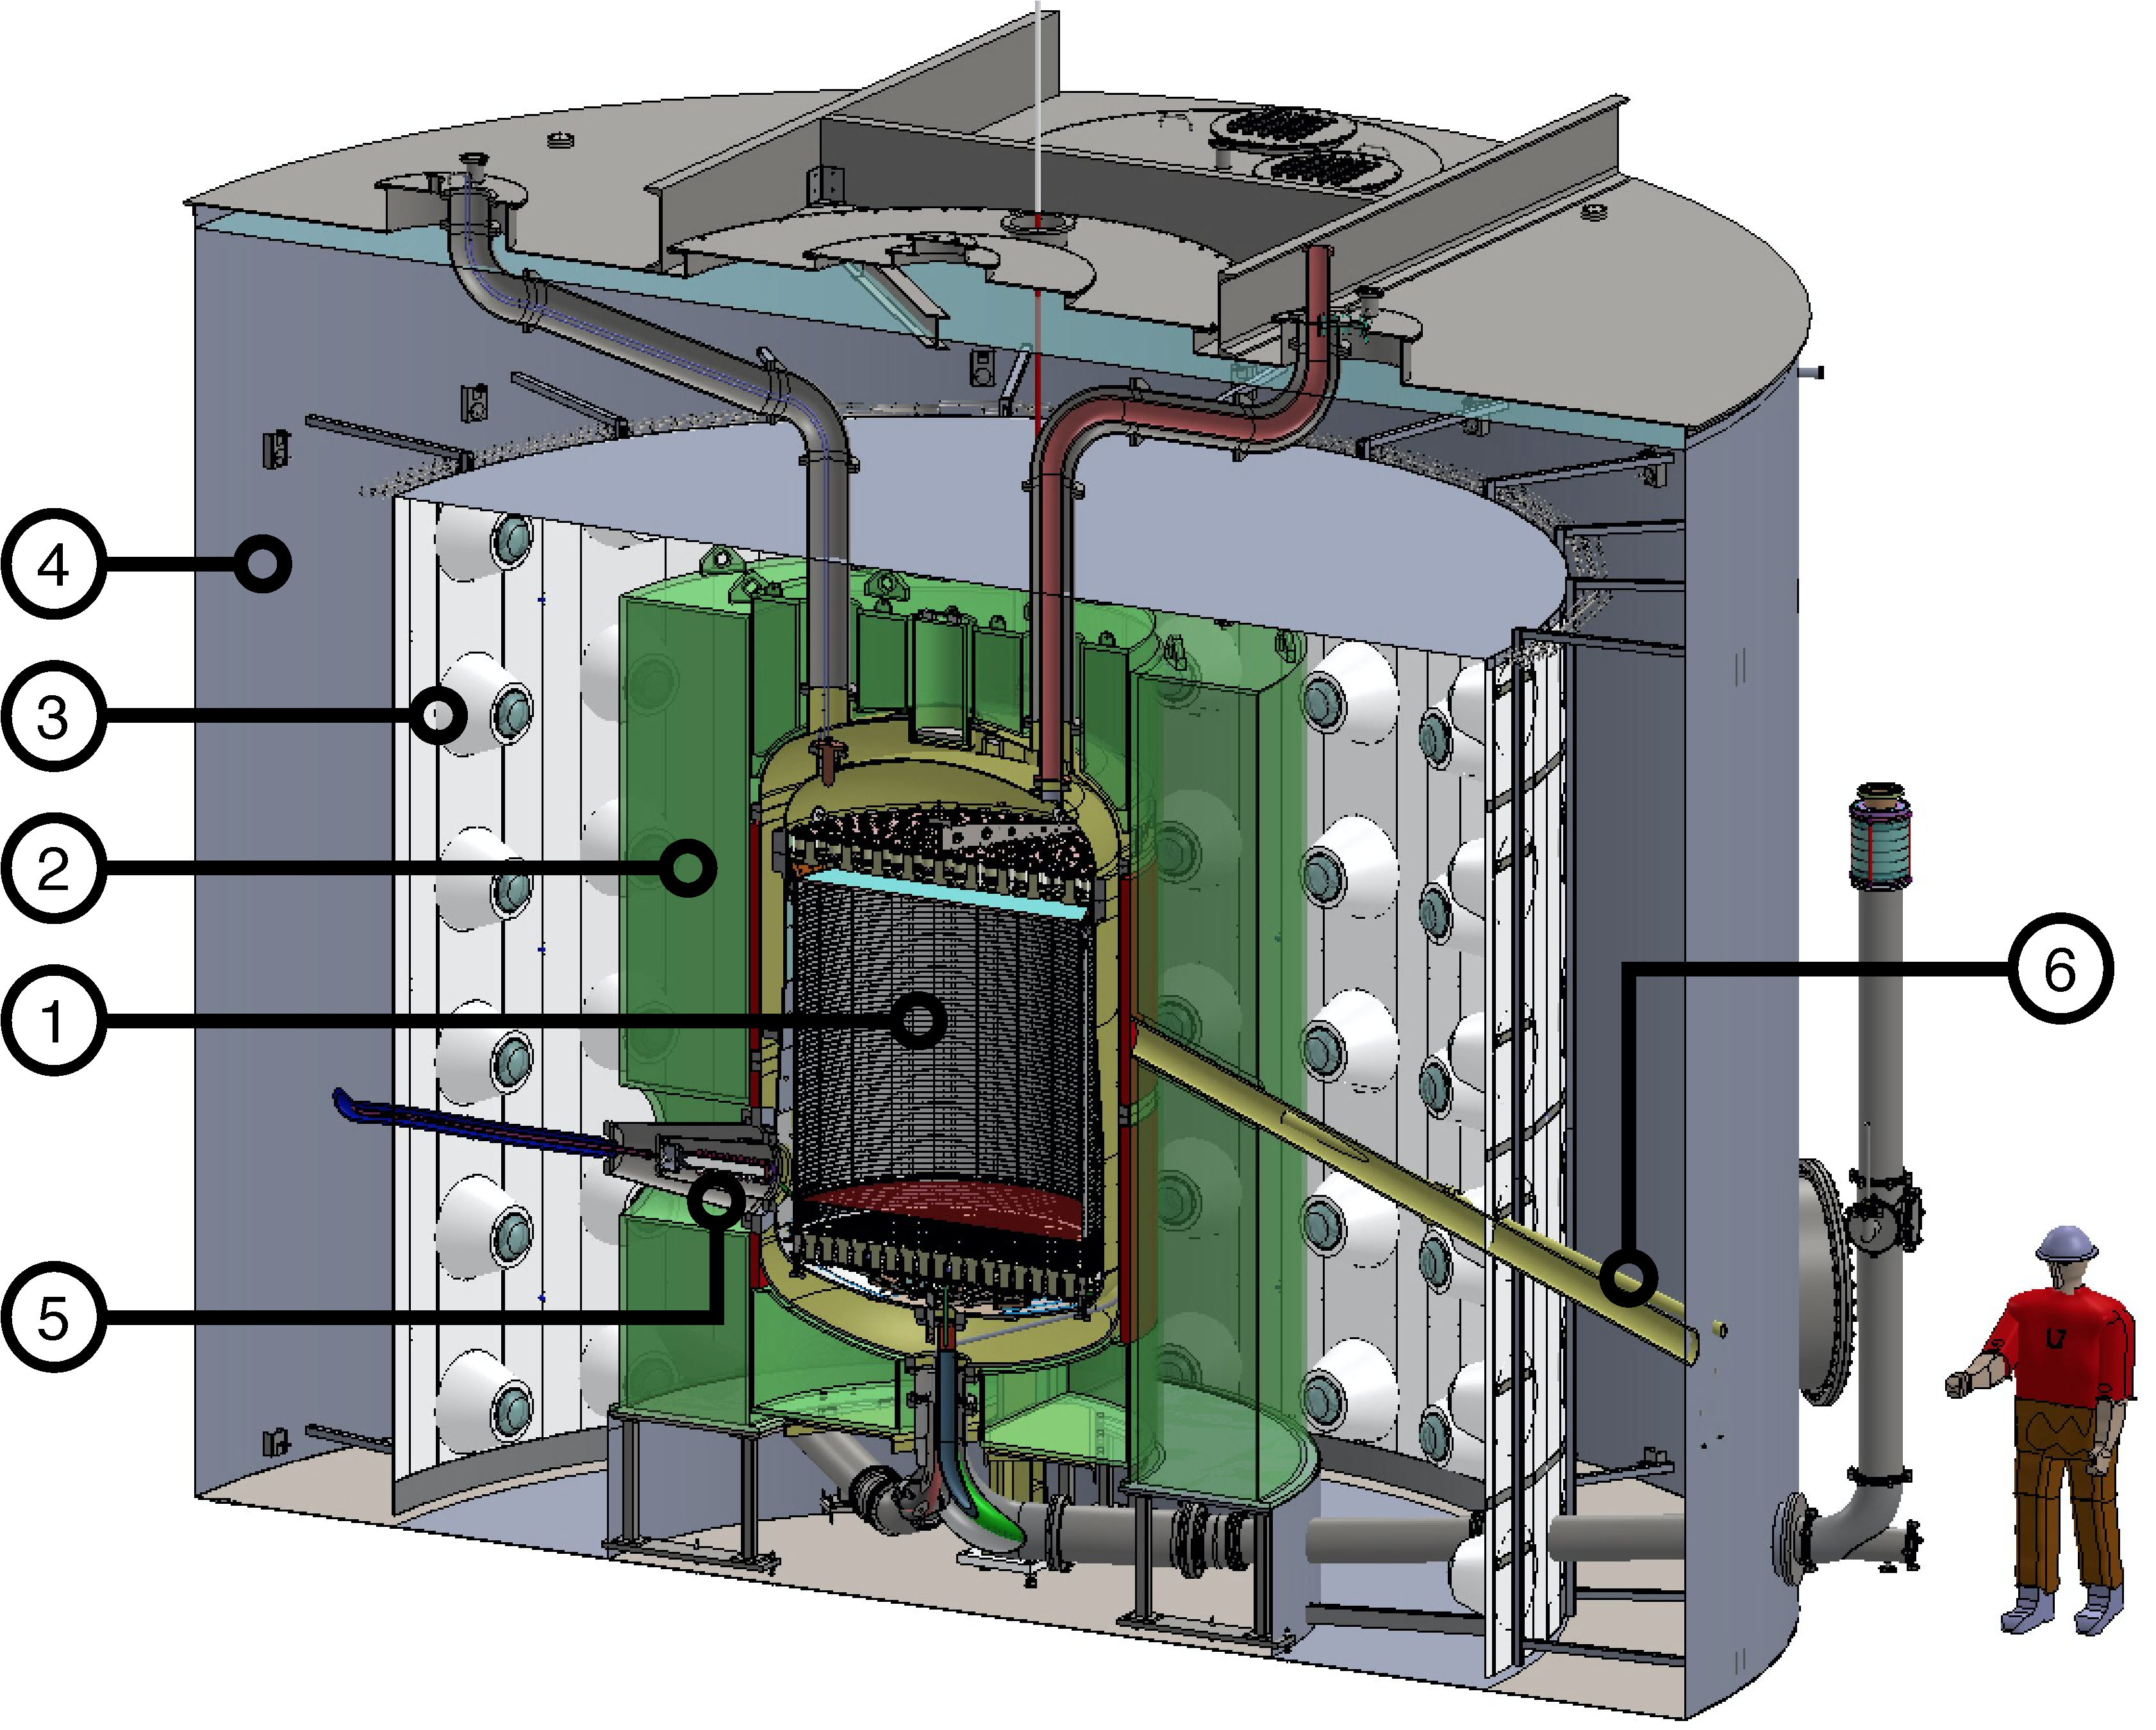
\includegraphics[width=0.8\linewidth]{figures/LZ/LZSchematic.pdf}
    \caption{Schematic of the LZ detector showcasing the major subsystems. At the center is the liquid xenon TPC (1), monitored by two arrays of PMTs and serviced by various cable and fluid conduits (upper and lower). The TPC is contained in a double-walled vacuum insulated titanium cryostat and surrounded on all sides by a GdLS Outer Detector (2). The cathode high voltage connection is made horizontally at the lower left (5). The GdLS is observed by a suite of 8” PMTs (3) standing in the water (4) which provides shielding for the detector. The pitched conduit on the right (6) allows for neutron calibration sources to illuminate the detector \cite{LZNIMA}.}
    \label{fig:LZDetector}
\end{figure}
\section{Liquid Xenon Time Projection Chamber}
The LZ TPC holds 7~t (5.6~t fiducial) of liquid xenon (LXe) above its cathode, there is an additional thin layer (8~mm thick) of gaseous xenon (GXe) at the top of the liquid. The volume measures approximately 1.5~m in height and diameter and the walls of the TPC are made from PTFE to improve light collection efficiency \cite{LZNIMA}. The TPC, Skin and Xe payload are housed within the Inner Cryostat Vessel (ICV) and the Outer Cryostat Vessel (OCV) provides a vacuum jacket for insulation. Both cryostat vessels are made from low radioactivity titanium \cite{LZ:2017iwn}. When a particle scatters off a LXe atom a prompt scintillation signal (S1) is produced alongside free elections, via ionisation of the LXe atom. Through the application of an electric field, the free electrons drift to the LXe surface and are extracted in the GXe layer. As the electrons accelerate through the GXe layer, a proportional amount of scintillation light (S2) is produced. Light produced from these particle interactions is observed by a top and bottom array of 3-inch Hamamatsu R11410–22 PMTs, 494 in total. Using both the S1 and S2 signals, position reconstruction techniques can be used to determine the $xyz$-position of the particle interaction. The time difference between the S1 and S2 signals combined with the drift velocity is used to determine the $z$-position of the interaction whilst the hit pattern of the S2 signal in the top PMT array provides $xy$-position. This operating principle of a TPC can be seen in \autoref{fig:TPCCartoon}.
\begin{figure}
     \centering
     \begin{subfigure}[b]{0.5\textwidth}
         \centering
         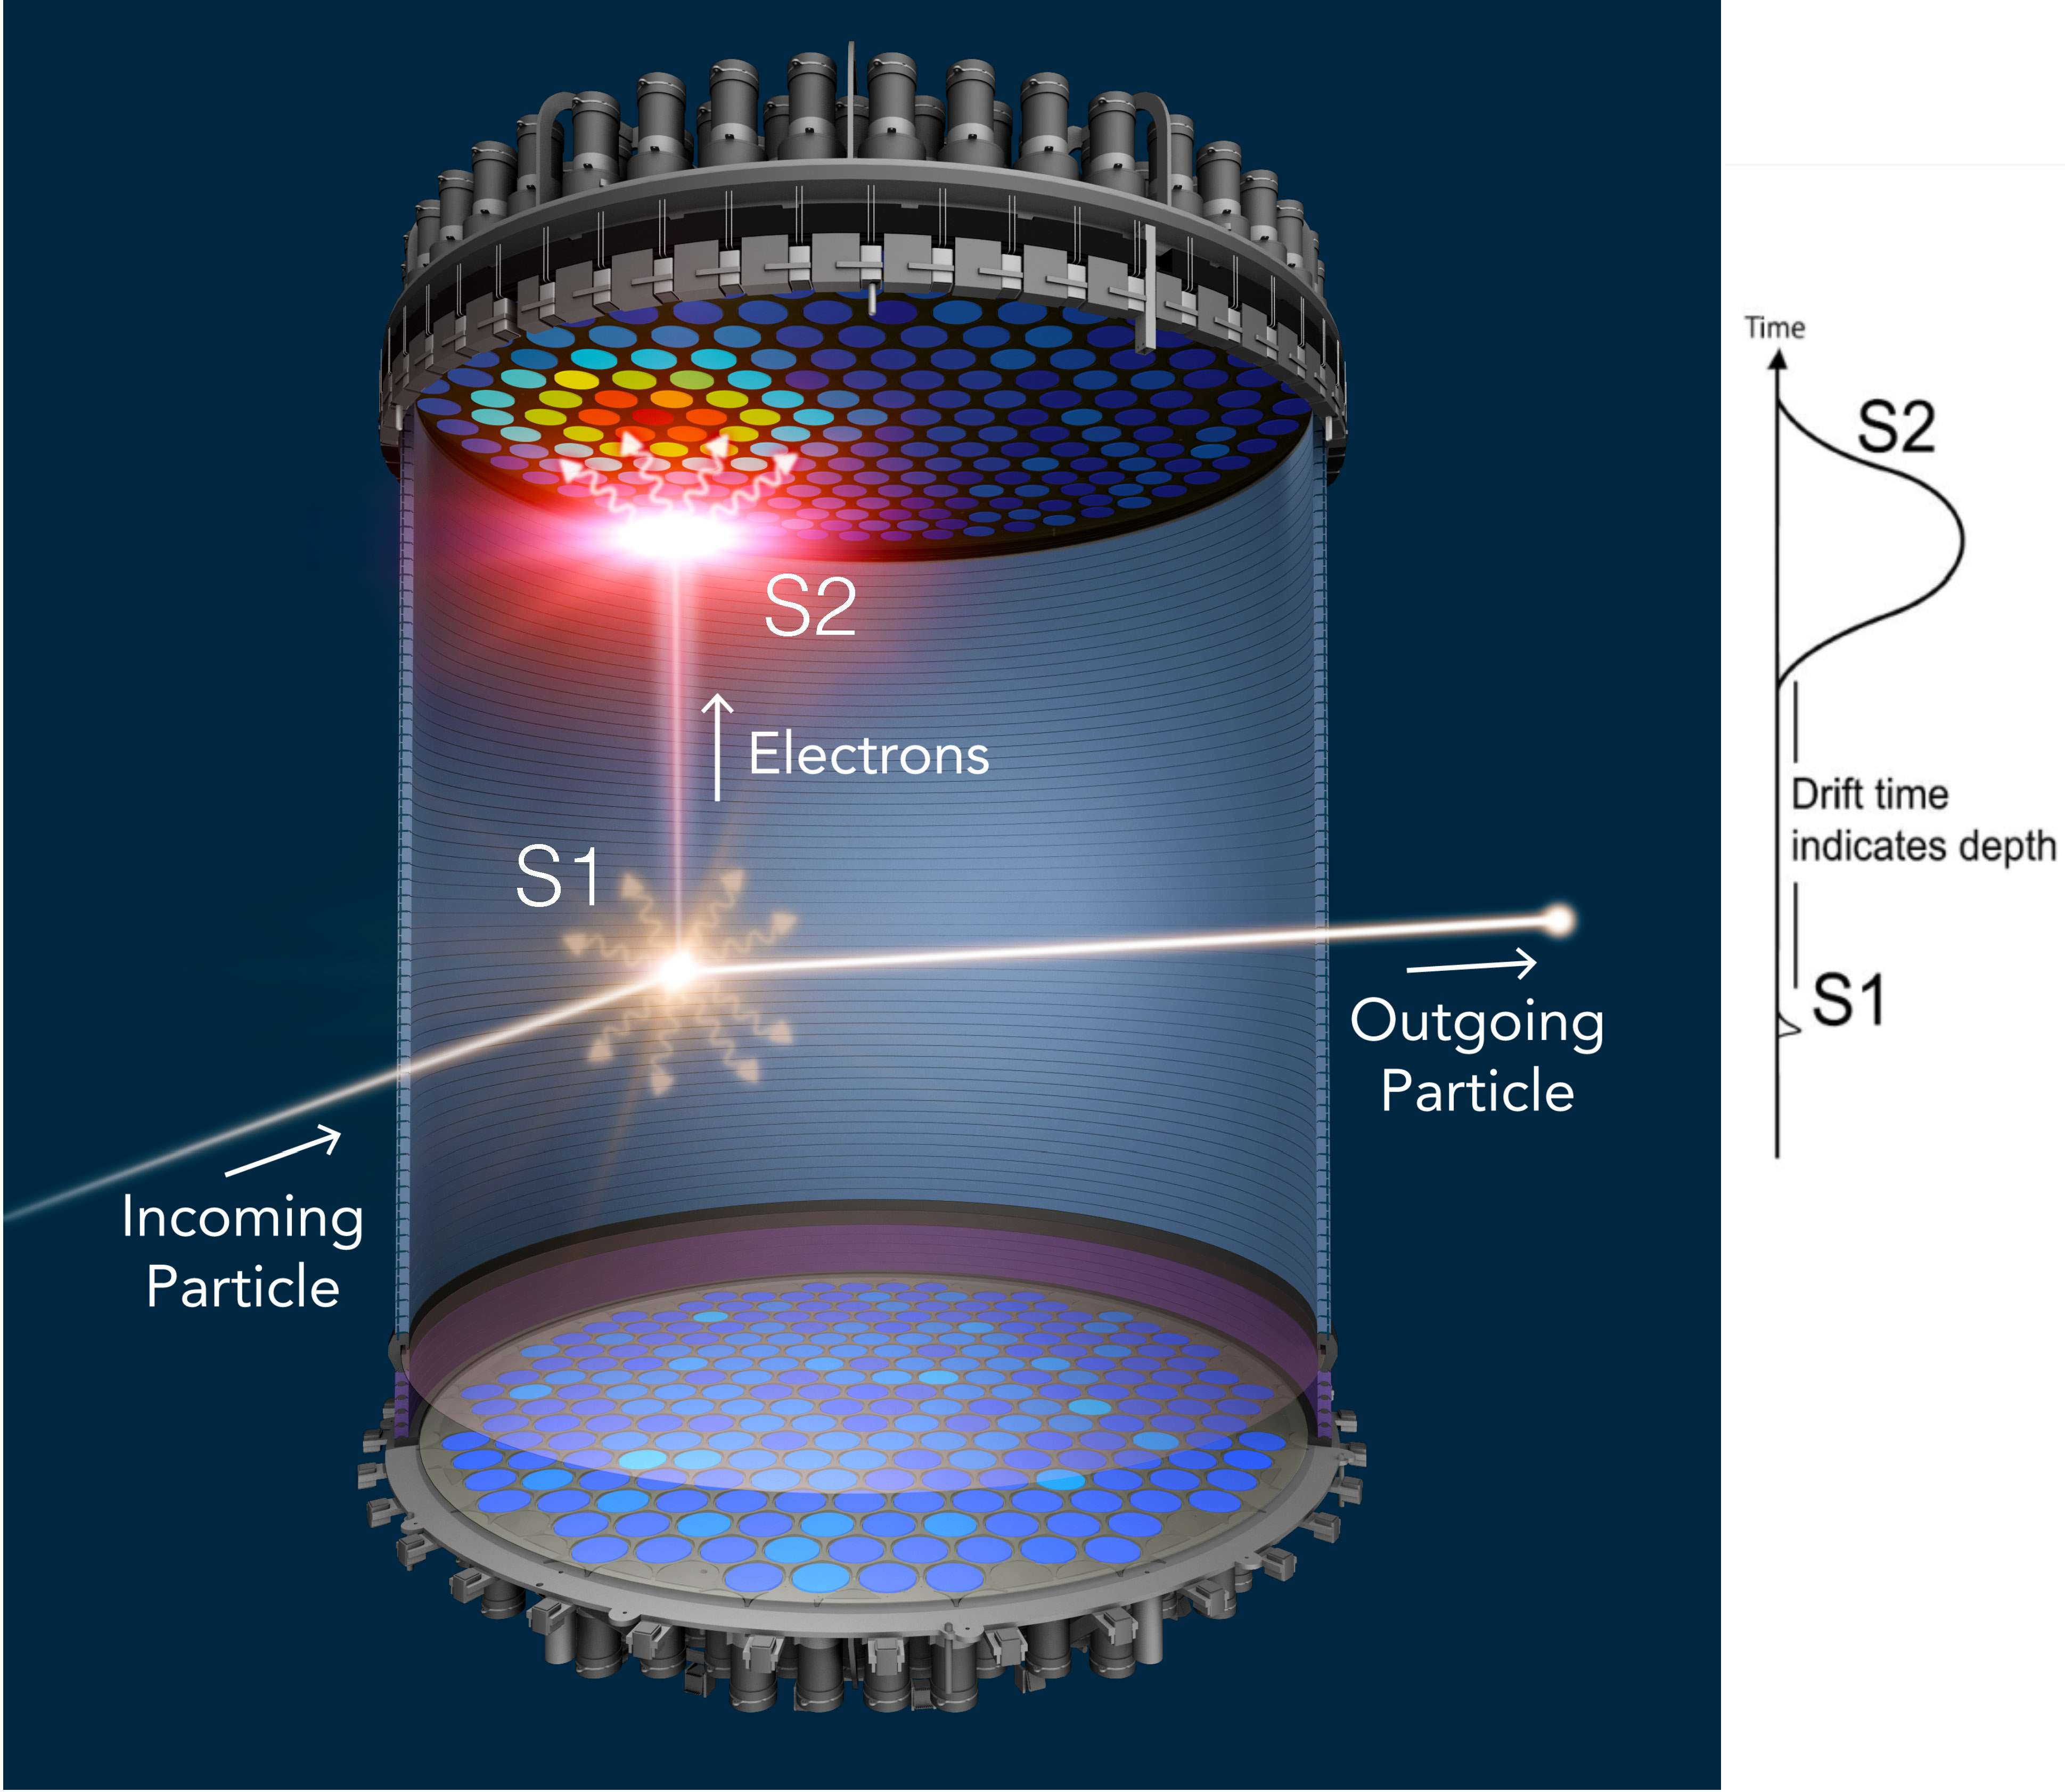
\includegraphics[width=\textwidth]{figures/LZ/IDOf_Xe_TPC2.jpg}
         \caption{Operating principle of a dual phase liquid noble TPC. \cite{LZTDR}}
         \label{fig:y equals x}
     \end{subfigure}
     \hfill
     \begin{subfigure}[b]{0.5\textwidth}
         \centering
         \includegraphics[width=\textwidth]{}
         \caption{$y=3\sin x$}
         \label{fig:three sin x}
     \end{subfigure}
\end{figure}

\subsection{Particle-Xenon interactions within a TPC}


\section{Xenon Skin}

\section{Outer Detector}
\subsection{Scintillator}
\subsection{PMT system}
\subsection{Optical Calibration System}

\section{Calibration Sources}

\section{Data Acquisition System}

\section{Simulation Techniques}

\section{Assembly and Operation of the LZ Detector}